\documentclass[../TST.tex]{subfiles}
\begin{document}
\begin{pproblem}
A resistance $R=\qty{2}{\ohm}$ and a nonlinear lightbulb are connected in parallel. They are connected to a battery of EMF $E=\qty{4}{V}$ and internal resistance $r=\qty{0.5}{\ohm}$. The I-V curve of the lightbulb is given in the table. Find the power dissipated at the lightbulb.

\begin{center}
\begin{tabular}{@{}ll@{}}
\toprule
$U,\,\mathrm{V}$     & $I,\,\mathrm{A}$     \\ \midrule
0.50 & 0.60 \\
1.00 & 1.00 \\
1.50 & 1.30 \\
2.00 & 1.55 \\
2.50 & 1.75 \\
3.00 & 1.90 \\ \bottomrule
\end{tabular}
  \end{center}
\end{pproblem}
\ifprob \else
	\begin{solution} Using Kirchoff's rules, we will find how the voltage across the lightbulb $U$ is related to the current $I$ passing through it. The resistance $R$ is connected in parallel to the lightbulb, so the voltage across it is also equal to $U$, and the current through it is $\frac{U}{R}$. The total current through the battery is therefore $I_\mathrm{tot}=I+\frac{U}{R}$. Then, the loop equation for the circuit is
		\begin{equation*}
	E-I_\mathrm{tot}r-U=0	
		,
		\end{equation*}
which is the same as
\begin{equation}
	I=\frac{E}{r}-\frac{R+r}{Rr}U= (\qty{8}{A})-(\qty{2.5}{\ohm^{-1}})\,U
.\label{IV}
\end{equation}
On the other hand, $I$ and $U$ must also follow the I-V curve of the lightbulb. The state of the lightbulb will then correspond to the point on the I-V curve which lies on \eqref{IV}:
\begin{center}
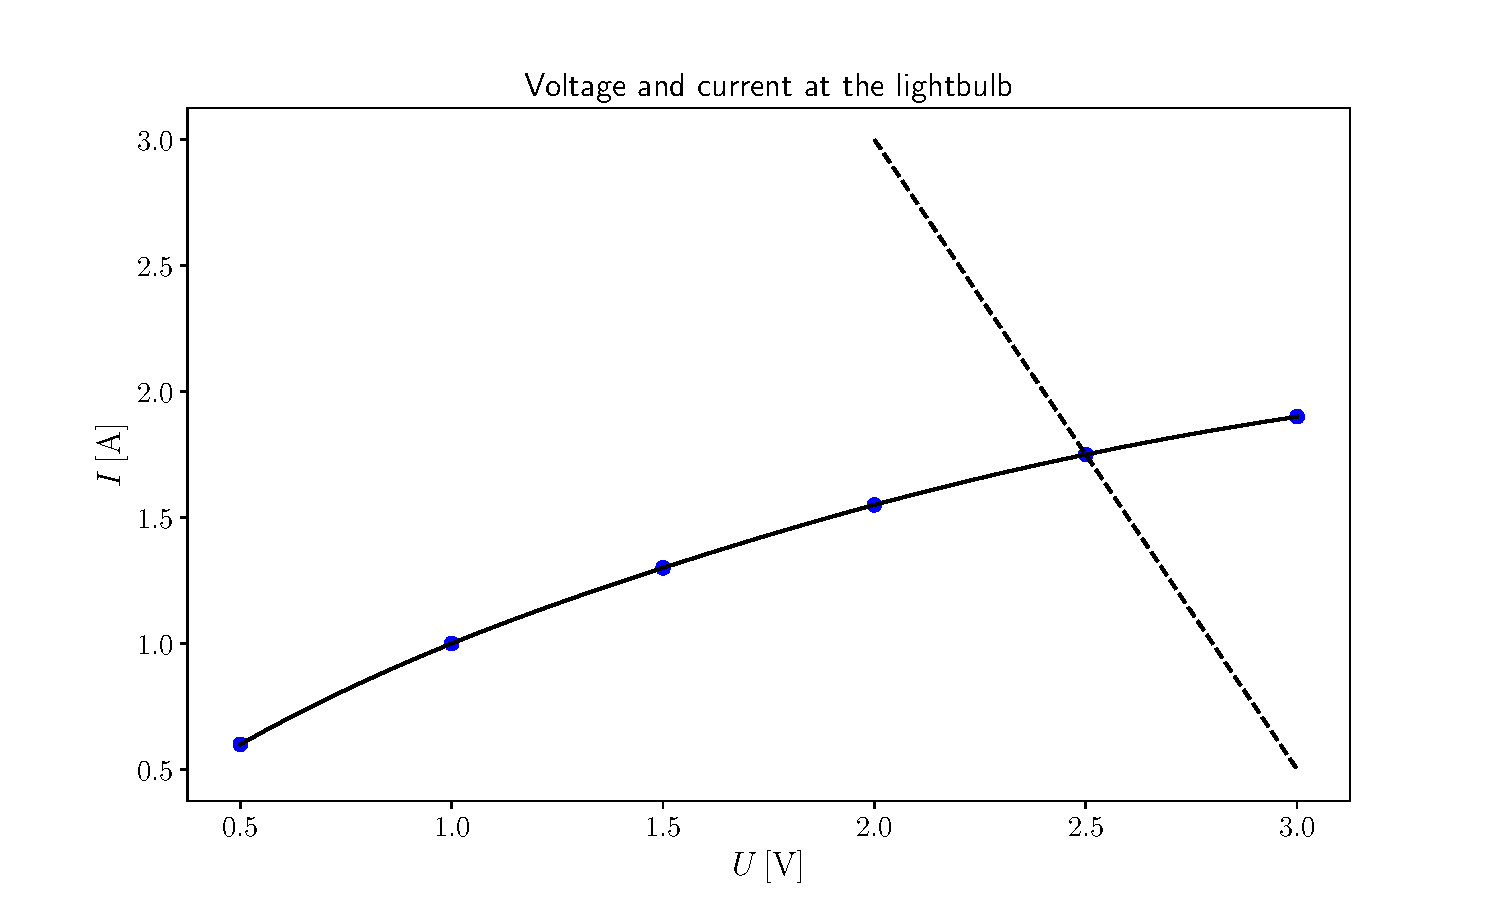
\includegraphics[width=0.9\textwidth]{fig/a2017_s4.pdf}
\end{center}
We find that the voltage is $U=\qty{2.50}{V}$, while the current is $I=\qty{1.75}{A}$. The dissipated power is $P=UI=\boxed{\qty{4.38}{W}}$.
\end{solution}
\fi
\end{document}
